\section*{Введение}
Цель работы – освоить новую для меня систему компьютерной верстки Latex, создать и грамотно оформить математический текст и таблицу с различными профессиями в области IT, - таблицу, отражающую желаемые мною вакансии, со всеми их плюсами и минусами.

\addcontentsline{toc}{section}{Введение}

\newpage
\section{Пример оформления математического текста}
Пусть функция $f$ определена в каждой точке интервала $(a, b)$, кроме, быть может, точки $x_0 \in (a, b)$.

\textbf {Определение 7.4} (определение предела по Гейне).
Число $A$ называется \textit{ пределом функции $f$ при стремлении
$x$ к $x_0$}, если для любой последовательности $\{x_n\}$ такой, что
$\{x_n\} \subset (a, b), \: x_n \neq x_0, \: x_n \rightarrow x_0, \: n \rightarrow \infty$, последовательность $f(x_n)$ значений функции $f$ сходится к $A$ при $n \rightarrow \infty$:

\begin{figure}[H]
\centerline{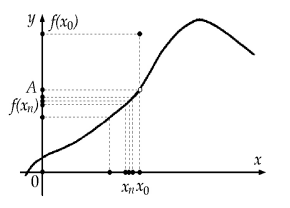
\includegraphics[width=0.5\linewidth]{pic1.png}}
\caption{Предел функции по Гейне}
\end{figure}

В этом случае пишут ~\eqref{f1}
\begin{equation}
\label{f1}
\centering
\lim_{x\to x_0} f(x)=A
\end{equation}

\textbf{Определение 7.5} (определение предела по Коши).
Число $A$ называется \textit{пределом функции $f$ при $x \rightarrow x_0$}, если ~\eqref{f2}

\begin{equation}
\label{f2}
\centering
\forall \epsilon >0 \; \; \exists \: \delta (\epsilon) >0 : \forall x \in (a,b) \rightarrow (0<|x-x_0|<\delta) \Rightarrow (|f(x)-A|<\epsilon).
\end{equation}

\begin{figure}[H]
\centerline{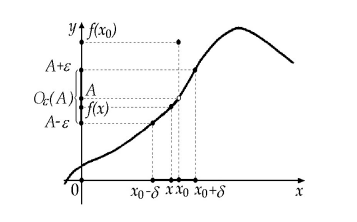
\includegraphics[width=0.6\linewidth]{pic2.png}}
\caption{Предел функции по Коши}
\end{figure}

\begin{theorem}
Определения предела функции по Гейне и по Коши эквивалентны.
\end {theorem} 
\begin {proof}
Докажем, что из определения по
Гейне следует определение по Коши. Проведем доказательство методом от противного.
\newline Пусть $\lim\limits_{x\to 0} f(x)=A$ по Гейне, но не по Коши, т. е. ~\eqref{f3}
\newline
\begin{equation}
\label{f3}
\centering
\exists \: \epsilon >0 \; \; \forall \: \delta (\epsilon) >0 \; \; \exists \: x_\delta \in (a, b) : (0<|x_\delta-x_0|<\delta \land |f(x_\delta)-A|\geq \epsilon).
\end{equation}
\newline
Пусть $\delta = \frac{1}{n}$. Тогда найдутся $x_n \in (a, b)$ такие, что ~\eqref{f4}
\newline
\begin{equation}
\label{f4}
\centering
0<|x_n-x_0|<\frac{1}{n}, \: |f(x_n)-A|\geq \epsilon
\end{equation}
\newline
Отсюда $x_n \neq x_0, \; x_n \rightarrow x_0$ но $f(x_n) \nrightarrow A$, что противоречит тому, что $f(x_n) \rightarrow A$ по Гейне.
\newline \indent Теперь докажем, что из определения предела по Коши
следует определение предела по Гейне.
\newline \indent \vspace{2mm} Пусть $\lim\limits_{x\to 0} f(x)=A$ по Коши. Возьмем любую последовательность $\{x_n\} \subset (a, b), \: x_n \rightarrow x_0, \: x_n \neq x_0$. Возьмем любое $\epsilon > 0$. Тогда из определения предела по Коши найдется $\delta > 0$, для которого, в силу сходимости $x_n \rightarrow x_0$, найдется номер $N$ такой, что $|x_n-x_0| < \delta$ при $n > N$. Тогда из
определения предела по Коши следует, что $|f(x_n)-A| < \epsilon$,
что означает, что $f(x_n) \rightarrow A$, т. е. $\lim\limits_{x\to 0} f(x)=A$ в смысле определения Гейне.
\end {proof}

\begin{theorem} \emph{Первая теорема Вейерштрасса.}
Если функция непрерывна на отрезке, то она ограничена на нем
\end {theorem} 
\begin {proof}
Пусть функция $f$ непрерывна на $[a, b]$. Необходимо доказать, что ~\eqref{f5}
\newline
\begin{equation}
\label{f5}
\centering
\exists \: M>0 : \forall x \in [a, b] \rightarrow |f(x)| \leq M
\end{equation}
\newline
Доказательство проведем методом от противного. Пусть
для каждого $M > 0$ найдется точка $x_M \in [a, b]$ такая, что
$|f(x_M)| > M$. Тогда для любого натурального $n$ найдется
$x_n \in [a, b]$ такая, что $|f(x_n)| > n$. Мы получим последовательность точек $\{x_n\} \subset [a, b]$, причем последовательность
значений функции $f(x_n) \rightarrow \infty$. Из ограниченности $\{x_n\}$
следует существование подпоследовательности $\{x_{n_k}\}$ такой, что $x_{n_k} \rightarrow c \in [a, b]$. Тогда из непрерывности функции
$f$ на отрезке $[a, b]$ и, в частности, в точке $c$ следует, что
$f(x_{n_k}) \rightarrow f(c)$, в то время как по построению $f(x_{n_k}) \rightarrow \infty$.
Полученное противоречие доказывает теорему.
\end{proof}

\indent
Вся информация взята из книги Гурьяновой К.Н. "Математический анализ" \cite{matan}
\newpage
\begin{landscape}
\section{Таблицы}
\vspace{5mm}
Таблица 2.1 – Программист
\begin{table}[H]
	\begin{center}
		\begin{small}
		\begin{tabular}{|p{1.1cm}|p{6cm}|p{5.2cm}|p{4cm}|p{4cm}|} \hline
			\multicolumn{1}{|c|}{№}&\multicolumn{1}{c|}{Наименование должности,}&\multicolumn{1}{c|}{Дисциплины из}&\multicolumn{1}{c|}{Преимущества }&\multicolumn{1}{c|}{Недостатки}\\ 
			\multicolumn{1}{|c|}{п.п.}&\multicolumn{1}{c|}{ссылка,зарплата}&\multicolumn{1}{c|}{учебного плана}&\multicolumn{1}{c|}{ вакансии}&\multicolumn{1}{c|}{вакансии}\\ 
			\hline
			1 & Инженер-программист С$\#$
			
			\url{https://clck.ru/32B7L9}
			
			до 180 000 т.р & Линейная алгебра, математический анализ, программирование, иностранный язык.& Бесплатный кофе/чай, оплачиваемые сверхурочные.& Опыт работы от 3 лет.\\
			\hline
			2 & Ведущий программист 1С
			
			\url{https://clck.ru/32B7LS}
			
			от 180 000 т.р. & Программирование.& Высокая зарплата, молодой и дружный коллектив.& Опыт работы 3-6 лет, длинный перечень требований.\\
			\hline
                3 & Программист Delphi
			
			\url{https://clck.ru/32B7Ly}
			
			180 000 - 350 000 т.р. & Программирование.& Удаленная работа, высокая зарплата.& Опыт работы 3-6 лет, незнакомый язык программирования.\\
			\hline
			4 & Программист SQL
			
			\url{https://clck.ru/32B7Mk}
			
			от 140 000 т.р & Программирование.& Возможность карьерного роста, соцпакет.& Офис в центре города (долго добираться).\\
			\hline
			5 & Программист С++
			
			\url{https://clck.ru/32B7SL}
			
			от 100 000 т.р. & Линейная алгебра, математический анализ, дискретная математика, администрирование ОС Linux, администрирование сетей Windows, Иностранный язык.& Рядом с домом, выделяются премии за каждый выполненный проект.& Опыт работы от 2 лет, опыт разработки многопоточных приложений.\\
			\hline
		\end{tabular}
	\end{small}
	\end{center}
\end{table}
Вывод: высокооплачиваемая специальность (средняя зарплата от 180 тыс. рублей), чтобы свободно ориентироваться в задачах данного профиля, необходим опыт (в среднем, различным компаниям достаточно хотя бы 2-3 лет).
\end{landscape}

\begin{landscape}
Таблица 2.2 – Web-разработчик
\begin{table}[H]
	\begin{center}
		\begin{small}
		\begin{tabular}{|p{1.1cm}|p{6cm}|p{5.2cm}|p{4cm}|p{4cm}|} \hline
			\multicolumn{1}{|c|}{№}&\multicolumn{1}{c|}{Наименование должности,}&\multicolumn{1}{c|}{Дисциплины из}&\multicolumn{1}{c|}{Преимущества }&\multicolumn{1}{c|}{Недостатки}\\ 
			\multicolumn{1}{|c|}{п.п.}&\multicolumn{1}{c|}{ссылка,зарплата}&\multicolumn{1}{c|}{учебного плана}&\multicolumn{1}{c|}{ вакансии}&\multicolumn{1}{c|}{вакансии}\\ 
			\hline
			1 & Старший Node.js бэкенд разработчик
			
			\url{https://clck.ru/32B7eV}
			
			до 350 000 т.р & Администрирование ОС Linux, Web-программирование, программирование.& Удаленная работа, известная крупная компания.& Опыт работы от 4 лет.\\
			\hline
			2 & Младший веб разработчик
			
			\url{https://clck.ru/32B7eb}
			
			90 000 т.р. & Web-программирование.& Высшее образование не обязательно, коммерческий опыт написания кода необязателен, комфортный офис.& Не самая высокая зарплата, плотный график.\\
			\hline
                3 & Web Программист FrontEnd
			
			\url{https://clck.ru/32B7ej}
			
			120 000 - 165 000 т.р. & Алгоритмы и структуры данных, web-программирование.& Близко к дому.& Строгий отбор, плотный график.\\
			\hline
			4 & Web-разработчик C$\#$ / .NET
			
			\url{https://clck.ru/32B7f6}
			
			от 200 000 т.р & Web-программирование.& Можно без опыта работы, удаленная работа, свободный график.& Незнакомый язык программирования.\\
			\hline
			5 & Frontend Developer
			
			\url{https://clck.ru/32B7hC}
			
			120 000-200 000 т.р. & Web-программирование, иностранный язык.& Удаленная работа, ежегодная степендия.& \\
			\hline
		\end{tabular}
	\end{small}
	\end{center}
\end{table}
Вывод: данная специальность требует относительно обширных знаний различных дисциплин (см. столбец “Дисциплины из учебного плана”). Также довольно-таки высокооплачиваемая.
\end{landscape}

\begin{landscape}
Таблица 2.3 – Разработчик игр
\begin{table}[H]
	\begin{center}
		\begin{small}
		\begin{tabular}{|p{1.1cm}|p{6cm}|p{5.2cm}|p{4cm}|p{4cm}|} \hline
			\multicolumn{1}{|c|}{№}&\multicolumn{1}{c|}{Наименование должности,}&\multicolumn{1}{c|}{Дисциплины из}&\multicolumn{1}{c|}{Преимущества }&\multicolumn{1}{c|}{Недостатки}\\ 
			\multicolumn{1}{|c|}{п.п.}&\multicolumn{1}{c|}{ссылка,зарплата}&\multicolumn{1}{c|}{учебного плана}&\multicolumn{1}{c|}{ вакансии}&\multicolumn{1}{c|}{вакансии}\\ 
			\hline
			1 & Программист-разработчик игр
			
			\url{https://clck.ru/32B7nc}
			
			75 000 - 150 000 т.р & Программирование, линейная алгебра, математический анализ, дискретная математика, информатика, web-программирование.& Удаленная работа, гибкий график, работать нужно 60 часов в месяц.& Сдельная оплата.\\
			\hline
			2 & Junior C++ Game Developer
			
			\url{https://clck.ru/32B7np}
			
			от 75 000 т.р. & Программирование, иностранный язык, Администрирование ОС Linux.& Удаленная работа, гибкое начало рабочего дня..& Опыт работы с системой контроля версий Git.\\
			\hline
                3 & Unity Developer
			
			\url{https://clck.ru/328cjj}
			
			до 150 000 т.р. & Программирование.& Удаленная работа, система бонусов.& Требуется опыт в разработке игр.\\
			\hline
			4 & Frontend-разработчик игр на HTML5
			
			\url{https://clck.ru/32B7oQ}
			
			от 150 000 т.р & Программирование, web-программирование.& Перспектива релокации за границу.& Опыт работы с Canvas, WebG.\\
			\hline
			5 & Unity разработчик
			
			\url{https://clck.ru/32B7pU}
			
			от 140 000 т.р. & Программирование, иностранный язык, мобильные системы передачи данных.& Удаленная работа, есть возможность переехать за границу.& Опыт в мобильной разработке.\\
			\hline
		\end{tabular}
	\end{small}
	\end{center}
\end{table}
Вывод: на мой взгляд самая интересная специальность из желаемых, но требующая ещё более обширных знаний, нежели предыдущая. Зарплаты высокие, но ниже, чем у профилей в вышестоящих таблицах.
\newline
\indent
Вся информация взята с официального сайта "HeadHunter" \cite{headhunter}
\end{landscape}


\newpage
\section*{Заключение}
Цель работы достигнута. Результатом стал отчет, содержащий математический текст и таблицы с информацией об актуальных вакансиях в области программирования. Я научился работать с новыми для меня функциями приложения Word. В частности, оформлять математический текст, работать с таблицами. Также научился правильно оформлять курсовую работу или же отчет.
\addcontentsline{toc}{section}{Заключение}